\documentclass[12pt]{extbook}

% \usepackage[paperwidth=5.5in, paperheight=8.5in, margin=0.3in]{geometry}
% \usepackage[paperwidth=8.5in, paperheight=11in, margin=0.5in]{geometry}

\usepackage[paperwidth=5.5in, paperheight=8.5in,bindingoffset=0.3in,margin=0.8in]{geometry}

% Fonts and typography

%% Typography
\usepackage[no-math]{fontspec}
\defaultfontfeatures{Mapping = tex-text, Scale = MatchLowercase}

\usepackage{csquotes}

%% Fonts
\setmainfont{Adobe Garamond Pro}
\setsansfont{Adobe Garamond Pro}
\setmonofont[Mapping=tex-ansi]{Menlo}

%% Set Sans font in headings
% \usepackage{sectsty}
% \allsectionsfont{\sffamily}

%% Set polyglossia language
\usepackage{polyglossia}
\setdefaultlanguage{english}

% \usepackage[fontsize=16pt]{scrextend}

\usepackage{titlesec}
% \titleformat{\chapter}[display]
%   {\normalfont\sffamily\huge\bfseries\centering}
%   {\chaptertitlename\ \thechapter}{20pt}{\Huge}
\titleformat{\section}
  {\normalfont\sffamily\huge\bfseries\centering}
  {\thesection}{1em}{\Huge}
% \titlespacing*{\chapter}{0pt}{30pt}{20pt}

% \usepackage{titlesec}
% \titleformat{\chapter}[display]
% {\normalfont\huge\bfseries}{\centering\chaptertitlename\ \thechapter}{20pt}{\Huge}


% new page for every chapter
% \newcommand{\sectionbreak}{\clearpage}

% Page

%% Use full page in book style
% \usepackage{fullpage}

\usepackage{fancyhdr}
\pagestyle{fancy}
\fancyhf{}
\fancyhead{}
\fancyfoot{}
\renewcommand{\headrulewidth}{0.1pt}
% \headrulewidth 0.0pt
% \fancyfoot[C]{\thepage}
\fancyfoot[RO, LE] {\thepage}

%% Set line spacing
\usepackage{setspace}
\setstretch{1.2}

%% Disable paragraph indentation
\usepackage{parskip}

\usepackage{afterpage}

\newcommand\blankpage{%
    \null
    \thispagestyle{empty}%
    \addtocounter{page}{-1}%
    \newpage}


%% Start sections from new page
% \let\stdsection\section
% \renewcommand\section{\newpage\stdsection}

\usepackage[labelformat=empty]{caption}

% Images
\usepackage{graphicx}

\usepackage{pdfpages}


\usepackage{xcolor}

%% Tango color scheme
\definecolor{SkyBlue}{HTML}{3465A4}
\definecolor{DarkSkyBlue}{HTML}{204A87}

\definecolor{Plum}{HTML}{75507B}

\definecolor{ScarletRed}{HTML}{CC0000}

\definecolor{Aluminium1}{HTML}{EEEEEC}
\definecolor{Aluminium6}{HTML}{2e3436}

\definecolor{Black}{HTML}{000000}


\usepackage{listings}

\lstdefinelanguage{JavaScript}{
  keywords = {typeof, new, true, false, catch, function, return, null, catch, switch, var, if, in, while, do, else, case, break},
  % keywordstyle = \color{SkyBlue}\bfseries,
  ndkeywords = {class, export, boolean, throw, implements, import, this},
  % ndkeywordstyle = \color{Aluminium6}\bfseries,
  % identifierstyle = \color{Black},
  sensitive = false,
  comment = [l]{//},
  morecomment = [s]{/*}{*/},
  % commentstyle = \color{Plum}\ttfamily,
  stringstyle = \color{ScarletRed}\ttfamily,
  morestring = [b]',
  morestring = [b]"
}

\lstset{
  language = JavaScript,
  % backgroundcolor = \color{Aluminium1},
  extendedchars = true,
  basicstyle = \normalsize\ttfamily,
  showstringspaces = false,
  showspaces = false,
  tabsize = 1,
  breaklines = true,
  showtabs = false
}

%% Normal enumerates processing
% \usepackage{enumerate}

%% Disable section numbers
% \setcounter{secnumdepth}{0}

\renewcommand\thesection{\arabic{section}}

\begin{document}

  % Title page
  % \thispagestyle{empty}
  % \pagestyle{myheadings}
  % \vspace*{\fill}
  %   \begin{center}
  %     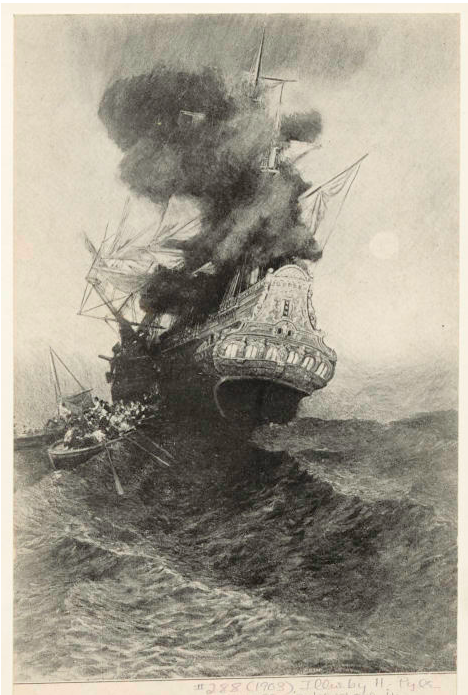
\includegraphics[width=0.98\textwidth]{img/title}
  %   \end{center}
  % \vspace*{\fill}

  % \begin{figure}
  % \noindent\makebox[\textwidth][c]{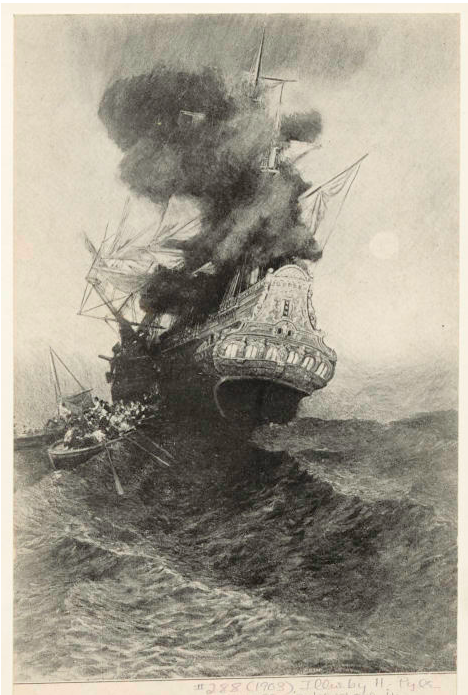
\includegraphics[width=1.4\textwidth]{img/title}}%
  % \end{figure}

  % \includepdf[pages={1}]{img/captain_z_title_2.pdf}

  \pagestyle{empty}
  \vspace*{\fill}
  \begin{center}
  \huge{Captain Z and the Treasure of Castle Island}\\[0.5cm]
  \end{center}
  \vspace*{\fill}
  % \afterpage{\blankpage}
  % \clearpage

  \begin{titlepage}
    \vspace*{\fill}
    \begin{center}
      \huge{Captain Z and the Treasure of Castle Island}\\[0.5cm]
      \large {Jim Vallandingham}\\[0.4cm]
    \end{center}
    \vspace*{\fill}
  % \clearpage
  \end{titlepage}
  
  \begingroup
  \footnotesize
  \parindent 0pt
  \parskip \baselineskip
  \vfill
  Captain Z and the Treasure of Castle Island \\
  Jim Vallandingham \\

  \vfill

  Copyright \textcopyright{} 2014 by Jim Vallandingham \\
  
  All rights reserved. No part of this publicatino may be reproduced, stored in a retrieval system, or transmitted in any form or by any means without prior consent of the copyright owners.

  For information about permission to reproduce selections from this book,\\
  write to Jim Vallandingham at 

  \begin{center}
    99 32 11 88 48 01\hspace{2em}9 9 8 6 5 4 %1 
  \end{center}

  \begin{center}
  \begin{tabular}{ll}
    First edition:  & May 2014
  \end{tabular}
  \end{center}

  \vfill
  \vspace*{2\baselineskip}
  \clearpage
  \endgroup

  \begingroup
  \vspace*{\fill}
  \begin{center}
  To my wife, daughter, and son.
  \end{center}
  \vspace*{\fill}
  \afterpage{\blankpage}
  \endgroup
  \setcounter{page}{0}
  \clearpage
  

  % \frontmatter
  
  \pagestyle{fancy}

  % Book contents
  $body$

\end{document}

